% Graphic for TeX using PGF
% Title: /home/satenske/Diagramme1.dia
% Creator: Dia v0.97.1
% CreationDate: Wed Nov 30 19:04:23 2011
% For: satenske
% \usepackage{tikz}
% The following commands are not supported in PSTricks at present
% We define them conditionally, so when they are implemented,
% this pgf file will use them.
\ifx\du\undefined
  \newlength{\du}
\fi
\setlength{\du}{15\unitlength}
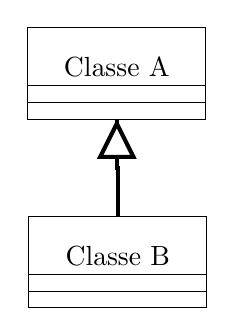
\begin{tikzpicture}
\pgftransformxscale{1.000000}
\pgftransformyscale{-1.000000}
\definecolor{dialinecolor}{rgb}{0.000000, 0.000000, 0.000000}
\pgfsetstrokecolor{dialinecolor}
\definecolor{dialinecolor}{rgb}{1.000000, 1.000000, 1.000000}
\pgfsetfillcolor{dialinecolor}
\pgfsetlinewidth{0.000000\du}
\pgfsetdash{}{0pt}
\definecolor{dialinecolor}{rgb}{1.000000, 1.000000, 1.000000}
\pgfsetfillcolor{dialinecolor}
\fill (20.250000\du,3.150000\du)--(20.250000\du,4.550000\du)--(24.542500\du,4.550000\du)--(24.542500\du,3.150000\du)--cycle;
\definecolor{dialinecolor}{rgb}{0.000000, 0.000000, 0.000000}
\pgfsetstrokecolor{dialinecolor}
\draw (20.250000\du,3.150000\du)--(20.250000\du,4.550000\du)--(24.542500\du,4.550000\du)--(24.542500\du,3.150000\du)--cycle;
% setfont left to latex
\definecolor{dialinecolor}{rgb}{0.000000, 0.000000, 0.000000}
\pgfsetstrokecolor{dialinecolor}
\node at (22.396250\du,4.100000\du){Classe A};
\definecolor{dialinecolor}{rgb}{1.000000, 1.000000, 1.000000}
\pgfsetfillcolor{dialinecolor}
\fill (20.250000\du,4.550000\du)--(20.250000\du,4.950000\du)--(24.542500\du,4.950000\du)--(24.542500\du,4.550000\du)--cycle;
\definecolor{dialinecolor}{rgb}{0.000000, 0.000000, 0.000000}
\pgfsetstrokecolor{dialinecolor}
\draw (20.250000\du,4.550000\du)--(20.250000\du,4.950000\du)--(24.542500\du,4.950000\du)--(24.542500\du,4.550000\du)--cycle;
\definecolor{dialinecolor}{rgb}{1.000000, 1.000000, 1.000000}
\pgfsetfillcolor{dialinecolor}
\fill (20.250000\du,4.950000\du)--(20.250000\du,5.350000\du)--(24.542500\du,5.350000\du)--(24.542500\du,4.950000\du)--cycle;
\definecolor{dialinecolor}{rgb}{0.000000, 0.000000, 0.000000}
\pgfsetstrokecolor{dialinecolor}
\draw (20.250000\du,4.950000\du)--(20.250000\du,5.350000\du)--(24.542500\du,5.350000\du)--(24.542500\du,4.950000\du)--cycle;
\pgfsetlinewidth{0.000000\du}
\pgfsetdash{}{0pt}
\definecolor{dialinecolor}{rgb}{1.000000, 1.000000, 1.000000}
\pgfsetfillcolor{dialinecolor}
\fill (20.280000\du,7.695000\du)--(20.280000\du,9.095000\du)--(24.562500\du,9.095000\du)--(24.562500\du,7.695000\du)--cycle;
\definecolor{dialinecolor}{rgb}{0.000000, 0.000000, 0.000000}
\pgfsetstrokecolor{dialinecolor}
\draw (20.280000\du,7.695000\du)--(20.280000\du,9.095000\du)--(24.562500\du,9.095000\du)--(24.562500\du,7.695000\du)--cycle;
% setfont left to latex
\definecolor{dialinecolor}{rgb}{0.000000, 0.000000, 0.000000}
\pgfsetstrokecolor{dialinecolor}
\node at (22.421250\du,8.645000\du){Classe B};
\definecolor{dialinecolor}{rgb}{1.000000, 1.000000, 1.000000}
\pgfsetfillcolor{dialinecolor}
\fill (20.280000\du,9.095000\du)--(20.280000\du,9.495000\du)--(24.562500\du,9.495000\du)--(24.562500\du,9.095000\du)--cycle;
\definecolor{dialinecolor}{rgb}{0.000000, 0.000000, 0.000000}
\pgfsetstrokecolor{dialinecolor}
\draw (20.280000\du,9.095000\du)--(20.280000\du,9.495000\du)--(24.562500\du,9.495000\du)--(24.562500\du,9.095000\du)--cycle;
\definecolor{dialinecolor}{rgb}{1.000000, 1.000000, 1.000000}
\pgfsetfillcolor{dialinecolor}
\fill (20.280000\du,9.495000\du)--(20.280000\du,9.895000\du)--(24.562500\du,9.895000\du)--(24.562500\du,9.495000\du)--cycle;
\definecolor{dialinecolor}{rgb}{0.000000, 0.000000, 0.000000}
\pgfsetstrokecolor{dialinecolor}
\draw (20.280000\du,9.495000\du)--(20.280000\du,9.895000\du)--(24.562500\du,9.895000\du)--(24.562500\du,9.495000\du)--cycle;
\pgfsetlinewidth{0.100000\du}
\pgfsetdash{}{0pt}
\pgfsetmiterjoin
\pgfsetbuttcap
{
\definecolor{dialinecolor}{rgb}{0.000000, 0.000000, 0.000000}
\pgfsetfillcolor{dialinecolor}
% was here!!!
\definecolor{dialinecolor}{rgb}{0.000000, 0.000000, 0.000000}
\pgfsetstrokecolor{dialinecolor}
\draw (22.396250\du,5.350269\du)--(22.396250\du,6.522500\du)--(22.421250\du,6.522500\du)--(22.421250\du,7.694731\du);
}
\definecolor{dialinecolor}{rgb}{0.000000, 0.000000, 0.000000}
\pgfsetstrokecolor{dialinecolor}
\draw (22.396250\du,6.262072\du)--(22.396250\du,6.522500\du)--(22.421250\du,6.522500\du)--(22.421250\du,7.694731\du);
\pgfsetmiterjoin
\definecolor{dialinecolor}{rgb}{1.000000, 1.000000, 1.000000}
\pgfsetfillcolor{dialinecolor}
\fill (22.796250\du,6.262072\du)--(22.396250\du,5.462072\du)--(21.996250\du,6.262072\du)--cycle;
\pgfsetlinewidth{0.100000\du}
\pgfsetdash{}{0pt}
\pgfsetmiterjoin
\definecolor{dialinecolor}{rgb}{0.000000, 0.000000, 0.000000}
\pgfsetstrokecolor{dialinecolor}
\draw (22.796250\du,6.262072\du)--(22.396250\du,5.462072\du)--(21.996250\du,6.262072\du)--cycle;
% setfont left to latex
\end{tikzpicture}
